\chapter{Numerical results}\label{ch:numerical_results}
In this chapter, after a short description of the class with manage the dumping on file, we report some simulation obtained with the code. Firstly we perform a simple simulation of a test problem to benchmark the code for what concern the solution of linear equations and, after that, we solve two particular cases of our problem that lead to a linear equation. Secondly we benchmark the non linear part of the code with a test case and than we solve our original problem with a quadratic source term.

\section{Dumping}\label{se:dump}
In the class \verb|output| there are implemented the methods to dump the result on file. The constructor accept two pointers: one which points to the mesh and one which points to the plasma state. The classes structure is shown in Fig.(\ref{fig:output_diagram}).
\begin{figure}
\centering
\subfigure{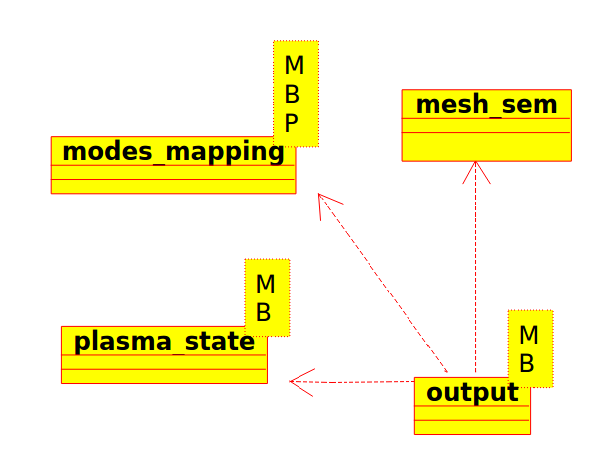
\includegraphics[scale=0.4]{images/output_diagram.png}}
\caption{Dumping: classes structure.}\label{fig:output_diagram}
\end{figure}

The class \verb|output| has three methods to perform the dump on file:
\begin{itemize}
  \item \verb|gmsh_dump(file_name)|: this method write, for each process, a file which contains the local portion of the mesh and the nodal values of the solution using the \verb|GMSH| format.
  \item \verb|dump(file_name,all_values)|: this method write, for each process, a file with contains, for each row, the $x$ coordinate, the $y$ coordinate and the value $\psi_{\delta}(x,y)$. If \verb|all_values| is set to \verb|false| only the nodal values are dumped, otherwise it sample for each elements the values of the solution on a structured mesh defined on the logical element. The sample points are equispaced and their number, for each element, is $(\max_m(p_m)+1\big)^2$. The points shared among different elements are write only once.
  \item \verb|dump_binary(file_name,all_values)|: this method is the same of \verb|dump| but, instead of using a unique file, it dumps the $x$ coordinate, the $y$ coordinate and the value $\psi_{\delta}(x,y)$ in three different files and the data are stored in binary format.
\end{itemize}

The solution values are extracted using the methods \verb|get_nodal_value(j)| and \verb|get_sol(j)| of the class \verb|plasma_state|.
\medskip

The class \verb|plasma_state| stores the values of the solutions. The nodal values are stored in a vector while a matrix stores in each row the coordinates and the values of the solution at that point. These two data structures are filled using the method \verb|update(n)| where \verb|n| is the number of points in which we want to split the edge. Therefore if it is equal to 0 we are taking only the nodal values of the solution while if it is equal to 1 we are taking the 4 nodal values, 4 values in the middle of each edge and 1 value in the center of the square. These values are evaluated using the method \verb|u_sol(x,y,e)| of the class \verb|modes_mapping|.
\medskip

In the following we report some plots of our simulations. The two-dimensional plots are the one obtained with \verb|GMSH| therefore they contains only the nodal values of the solution. Instead the surface plots are obtained using \verb|MATLAB| therefore they contain also the higher modes. Since the surfce plots function of \verb|MATLAB| deals only with structured grid, we project our solution over a structured grid using a linear interpolation and than we plot that solution.

\section{Examples}\label{sec:exemples}
The aim of these simulations is to test the code in different situations to benchmark it, therefore the emphasis of the analysis is not on the physical interpretation of the results obtained. All the tests were run on a small cluster using 8 processes. The basis degree is 2 for each variable and it is equal in all the elements. The dimension of the mesh is also very small, order of thousands of elements, therefore we refined the initial partition 5 times that is more than sufficient with so small mesh. The time of computation change a lot from simulation to simulation since it is strongly dominated by the iterative linear solver and in some case the stiffness matrix is very bad conditioned; it ranges from less than 1 second up to hundreds of seconds on the small cluster used.

\subsection{Benchmark linear test case: Poisson equation}\label{subsec:ex_poisson}
We choose to benchmark the linear part of our code with the well known Poisson equation in the domain $[-1,1]\times[-1,1]$. More precisely we want to solve the following linear problem
\begin{equation}
  \begin{cases}
   -\Delta u=(1-x^2)(1-y^2)& \mathrm{in}\:\Omega\\
   u=0& \mathrm{on}\:\partial\Omega
  \end{cases}
\end{equation}
which has solution the following analytical solution
\begin{equation}
 u(\mathbf{x})=-2x^2-2y^2+4.
\end{equation}

The discrete formulation of the problem is
\begin{equation}
  \begin{split}
    &\sum_m \bigg\{\sum_j \psi_j \sum_n w_n\:\hat{\nabla}\hat{\phi}_j(\mathbf{\hat{x}}_n)J_{\mathbf{F}_m}^{-1}(\mathbf{\hat{x}}_n)J_{\mathbf{F}_m}^{-T}(\mathbf{\hat{x}}_n)\hat{\nabla}\hat{\phi}_i(\mathbf{\hat{x}}_n)|\det(J_{\mathbf{F}_m}(\mathbf{\hat{x}}_n))|\bigg\}=\\
    &=0, \qquad\forall i\in\mathcal{I}
  \end{split}
\end{equation}
and is defined in the class \verb|poisson.h|.
\medskip

The mesh used is a structured one and it consists 4096 elements and 4230 nodes. The linear solver is the one used by default by \verb|PETSc|, the GMRES iterative method, while the preconditioner is the matrix itself with the flag \verb|DIFFERENT_NONZERO_PATTERN| which means that the preconditioning matrix does not have the same nonzero pattern structure during successive linear solves. We set two tolerances to test the convergence of the method: $10^{-15}$ for the decrease of the residual norm relative to the norm of the right hand side and for the absolute size of the residual norm while for the relative increase in the residual we set \verb|PETSC_DEFAULT|. Finally the maximum number of iterations is $10^4$. The plots of the numerical solution are reported in Fig.(\ref{fig:poisson}).

\begin{figure}
\centering
\subfigure{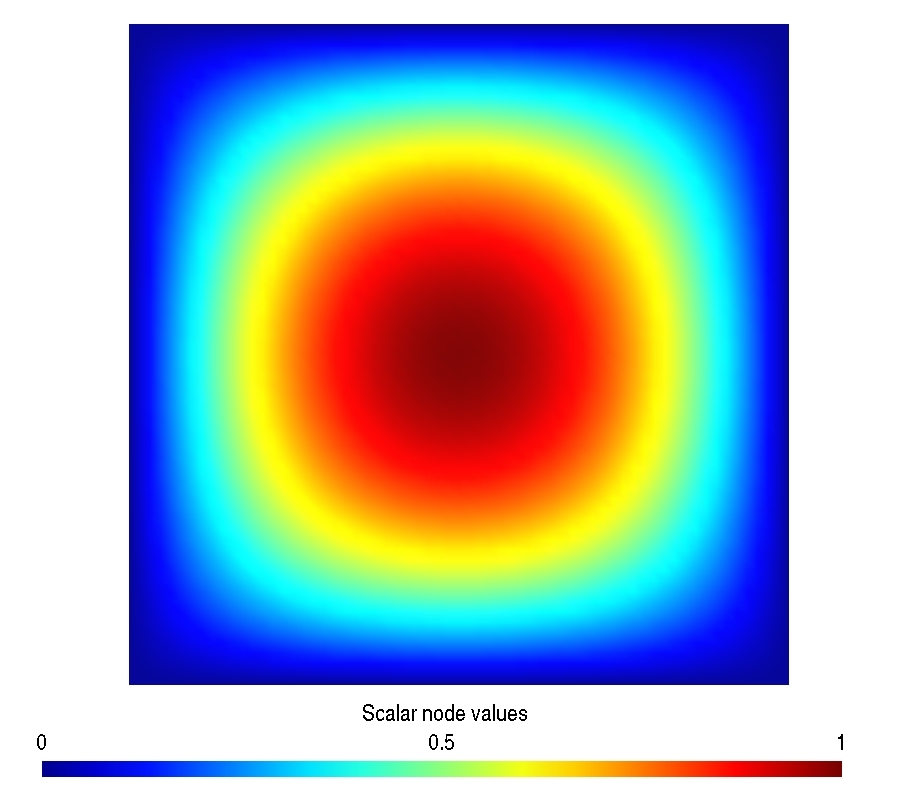
\includegraphics[scale=0.2]{images/poisson.jpg}}
\subfigure{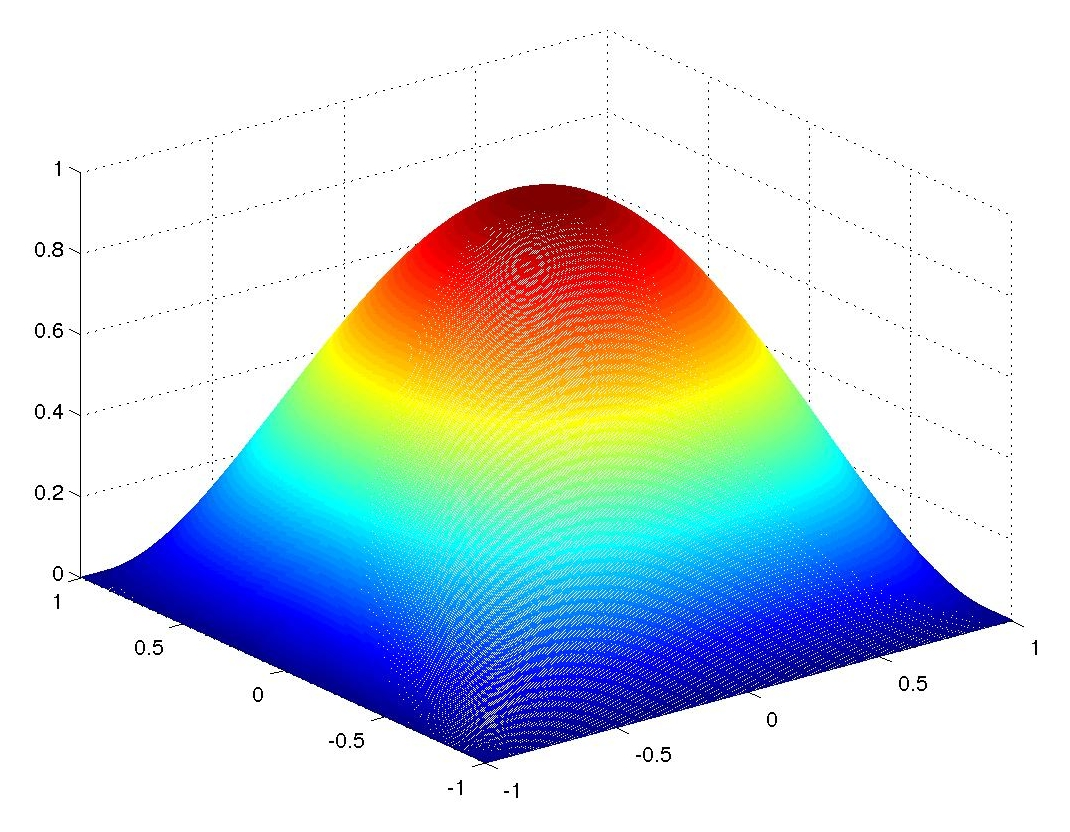
\includegraphics[scale=0.2]{images/poisson_surf.jpg}}
\caption{Discrete solution of the Poisson equation.}\label{fig:poisson}
\end{figure}

Since the analytical solution is a second order polynomial, in each variable,  we aspect to reach the precision of the machine since we are using a second order basis and Gaussian quadrature formula exact to the second order. This is indeed the case since
\begin{equation}
\|\mathbf{u}-\mathbf{u}_{\delta}\|_{\infty}=1.0170\cdot 10^{-13}
\end{equation}
where $\mathbf{u}$ is the vector of the exact solution evaluated in the points used to plot the surface while $\mathbf{u}_{\delta}$ are the discrete ones. This result tell us that the code works fine in the test case.

\subsection{Solution of the Grad-Shavranov operator}\label{subsec:ex_gs_operator}
We start to solve our problem, cmp. Eq.(\ref{eq:compact_equlibrium}), in the mirror domain shown in Fig.(\ref{fig:mirror_domain}) with the following parallel pressure profile
\begin{equation}
  p_{\|}(\psi,B)=0.
\end{equation}
Using this profile we obtain
\begin{equation}
  \begin{cases}
    \mathbf{F}(r,z,B,\psi,\nabla B, \nabla\psi)=0\\
     f(r,z,B,\psi)=0
  \end{cases}
\end{equation}
and the problem (\ref{eq:compact_equlibrium}) becomes
\begin{equation}
  \begin{cases}
    -\Delta^*\psi=0 & \mathrm{in}\:\Omega\\
    \psi(z,\gamma(z))=2\\
    \psi(0,r)=\psi(1,r)\\
    \nabla\psi(0,r)=\nabla\psi(1,r)
  \end{cases}
\end{equation}
which is linear. The discrete formulation of the problem is
\begin{equation}
  \begin{split}
    &\sum_m \bigg\{\sum_j \psi_j \sum_n w_n\:\mathbf{F}_m^r(\mathbf{\hat{x}}_n)\hat{\nabla}\hat{\phi}_j(\mathbf{\hat{x}}_n)J_{\mathbf{F}_m}^{-1}(\mathbf{\hat{x}}_n)J_{\mathbf{F}_m}^{-T}(\mathbf{\hat{x}}_n)\hat{\nabla}\hat{\phi}_i(\mathbf{\hat{x}}_n)|\det(J_{\mathbf{F}_m}(\mathbf{\hat{x}}_n))| +\\
    &+2\:\sum_j\psi_j\sum_n w_n[\frac{\partial\hat{x}}{\partial r},\frac{\partial\hat{y}}{\partial r}]_{\big|_{\mathbf{\hat{x}}_n}}\hat{\nabla} \hat{\phi}_j(\mathbf{\hat{x}}_n)\:\hat{\phi}_i(\mathbf{\hat{x}}_n)|\det(J_{\mathbf{F}_m}(\mathbf{\hat{x}}_n))|\bigg\}=0, \qquad\forall i\in\mathcal{I}
  \end{split}
\end{equation}
and is defined in the class \verb|lineargradshavranov.h|.
\medskip

The mesh used is an unstructured one and it consists of 2250 elements and 2159 nodes; we used the algorithm frontal of \verb|GMSH| starting from a boundary discretized with 92 nodes. The settings of the linear solver are the same of the ones used in the benchmark of the nonlinear problem, cmp.(\ref{subsec:ex_poisson}).The plots of the numerical solution are reported in Fig.(\ref{fig:gs_linear}).

\begin{figure}
\centering
\subfigure{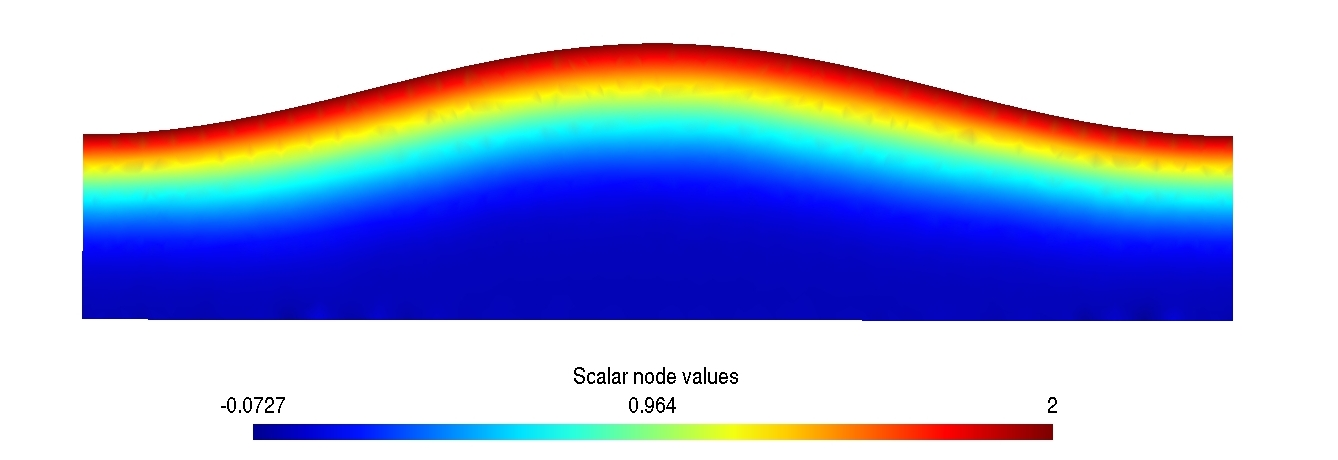
\includegraphics[scale=0.3]{images/gs_linear_nbc.jpg}}
\subfigure{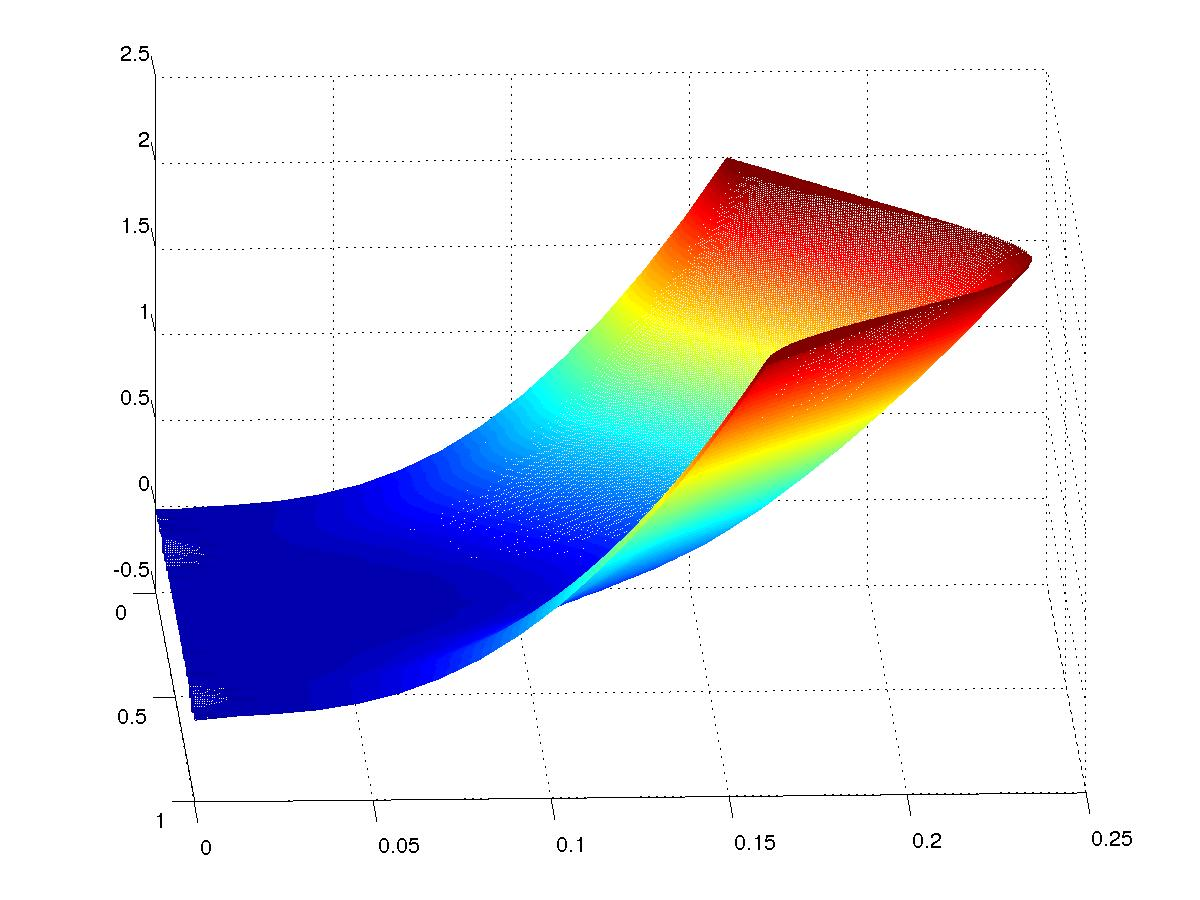
\includegraphics[scale=0.3]{images/gs_linear_nbc_surf.jpg}}
\caption{Discrete solution of the Grad-Shavranov operator.}\label{fig:gs_linear}
\end{figure}

The variable $\psi$ has not significant physical meaning itself indeed it is just a label for the magnetic field lines. Therefore the solution plotted in Fig.(\ref{fig:gs_linear}) represent the shape of the magnetic field lines in the special case of absence of parallel pressure.
\newpage

\subsection{Liner Grad-Shavranov problem}
We now solve our problem, cmp. Eq.(\ref{eq:compact_equlibrium}), in the inner tokamak domain with the following parallel pressure profile
\begin{equation}
  p_{\|}(\psi,B)=\frac{\partial}{\partial\psi}\bigg(p_0\big(1-\frac{\psi^2}{\psi_0^2}\big)\bigg).
\end{equation}
Using this profile we obtain
\begin{equation}
  \begin{cases}
    \mathbf{F}(r,z,B,\psi,\nabla B, \nabla\psi)=0\\
     f(r,z,B,\psi)=-2\frac{p_0}{\psi^2_0}\psi
  \end{cases}
\end{equation}
and the problem (\ref{eq:compact_equlibrium}) becomes
\begin{equation}
  \begin{cases}
    -\Delta^*\psi+2\frac{p_0}{\psi^2_0}r^2\psi=0 & \mathrm{in}\:\Omega\\
    \psi(z,\gamma(z))=2\\
    \psi(0,r)=\psi(1,r)\\
    \nabla\psi(0,r)=\nabla\psi(1,r)
  \end{cases}
\end{equation}
which is linear. The discrete formulation of the problem is
\begin{equation}
  \begin{split}
    &\sum_m \bigg\{\sum_j \psi_j \sum_n w_n\:\mathbf{F}_m^r(\mathbf{\hat{x}}_n)\hat{\nabla}\hat{\phi}_j(\mathbf{\hat{x}}_n)J_{\mathbf{F}_m}^{-1}(\mathbf{\hat{x}}_n)J_{\mathbf{F}_m}^{-T}(\mathbf{\hat{x}}_n)\hat{\nabla}\hat{\phi}_i(\mathbf{\hat{x}}_n)|\det(J_{\mathbf{F}_m}(\mathbf{\hat{x}}_n))| +\\
    &+2\:\sum_j\psi_j\sum_n w_n[\frac{\partial\hat{x}}{\partial r},\frac{\partial\hat{y}}{\partial r}]_{\big|_{\mathbf{\hat{x}}_n}}\hat{\nabla} \hat{\phi}_j(\mathbf{\hat{x}}_n)\:\hat{\phi}_i(\mathbf{\hat{x}}_n)|\det(J_{\mathbf{F}_m}(\mathbf{\hat{x}}_n))|+\\
    &+2\sum_n w_n\:\frac{p_0}{\psi^2_0}\mathbf{F}_m^r(\mathbf{\hat{x}}_n)^3 \hat{\phi}_j(\mathbf{\hat{x}}_n)\hat{\phi}_i(\mathbf{\hat{x}}_n)|\det(J_{\mathbf{F}_m}(\mathbf{\hat{x}}_n))|\bigg\}=0, \qquad\forall i\in\mathcal{I}
  \end{split}
\end{equation}
and is defined in the class \verb|lineargradshavranovmod.h|.
\medskip

The mesh used is an unstructured one and it consists 28752 elements and 28437 nodes; we used the algorithm Delaunay of \verb|GMSH| starting from a boundary discretized with 73 nodes and performing two refinements by splitting. The linear solver is the one used by default by \verb|PETSc|. No preconditioner has been used. We set two tolerances to test the convergence of the method: $10^{-15}$ for the decrease of the residual norm relative to the norm of the right hand side and for the absolute size of the residual norm while for the relative increase in the residual we set \verb|PETSC_DEFAULT|. Finally the maximum number of iterations is $10^4$. We choose $\frac{p_0}{\psi^2_0}=1$. The plots of the numerical solution are reported in Fig.(\ref{fig:gs_linear_mod}).

\begin{figure}
\centering
\subfigure{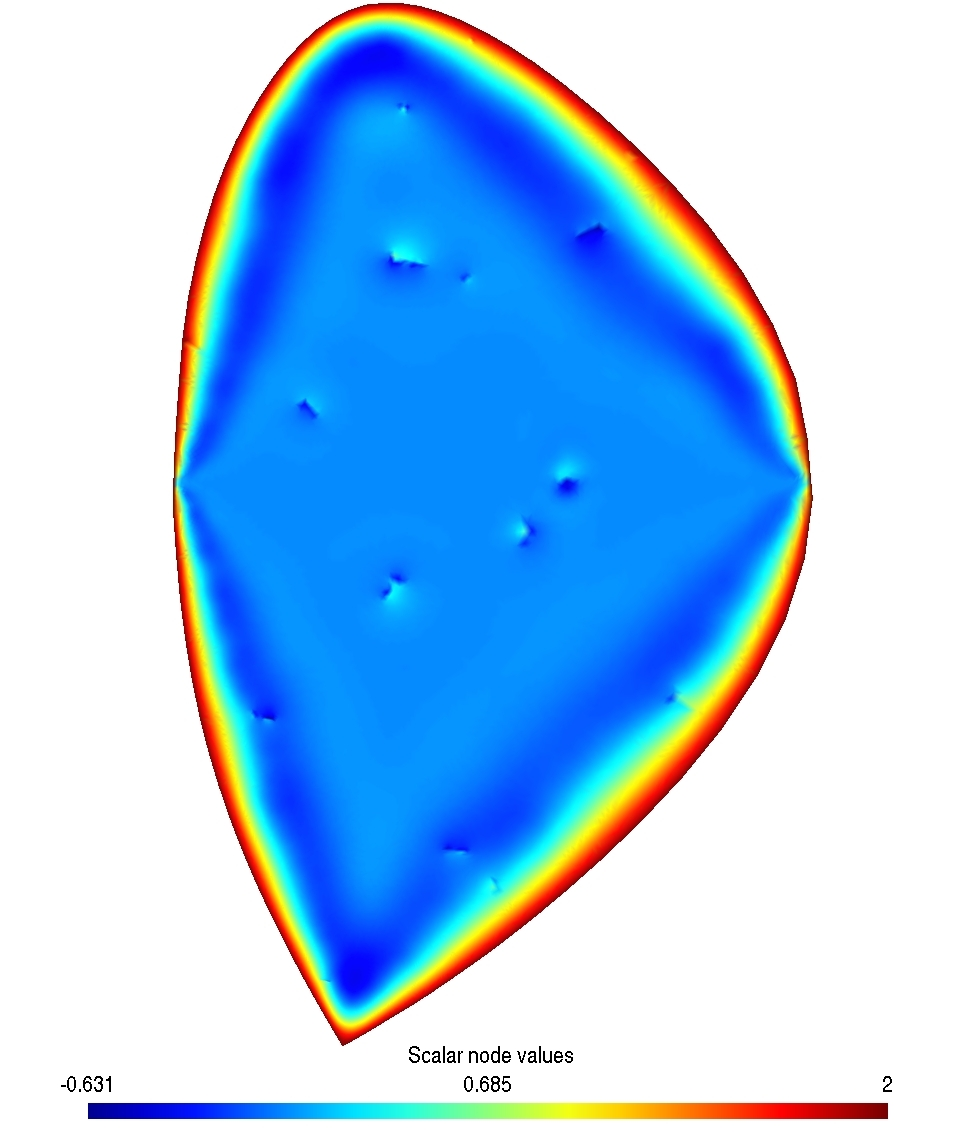
\includegraphics[scale=0.3]{images/gs_linear_mod_bis.jpg}}
\subfigure{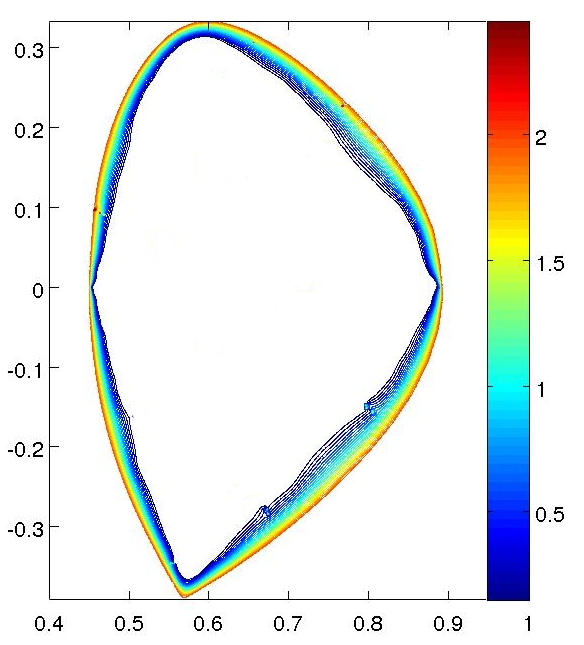
\includegraphics[scale=0.3]{images/gs_linear_mod_bis_countur.jpg}}
\caption{Discrete solution of the linear Grad-Shavranov problem and its countur plot.}\label{fig:gs_linear_mod}
\end{figure}

Unfortunately the problem is vary bad conditioned and the residual of the iterative solver decrease very slowly and it doesn't reach the tolerance requested also after all these iterations. We tried different preconditioner and different iterative solvers implemented in \verb|PETSc| but none of them works better. For this reason in Fig.(\ref{fig:gs_linear_mod}) we can see some noise due to the linear solver. We do not filtered it out to show where is localized the noise.

\subsection{Benchmark nonlinear test case: Bratu equation}
We choose to benchmark the nonlinear part of our code with the classical Bratu equation in the domain $[-1,1]\times[-1,1]$. More precisely we want to solve the following nonlinear problem
\begin{equation}
  \begin{cases}
   -\Delta u=\lambda e^{u}\qquad\mathrm{in}\:\Omega\\
   u=0\qquad\mathrm{on}\:\partial\Omega.
  \end{cases}
\end{equation}
Using the formalism introduced in Sec.(\ref{subsec:newton_method}) we have the following non linear functional $F$ defined as
\begin{equation}
  F(u)=\int_\Omega \big(\nabla u \cdot\nabla v-\lambda v\:e^{u}\big)\mathrm{d}\Omega
\end{equation}
and its Gateaux derivative is
\begin{equation}
  \mathcal{F}(u)\delta u=\int_\Omega \big(\nabla\delta u \cdot\nabla v-\lambda v\delta u\:e^{u}\big)\mathrm{d}\Omega.
\end{equation}

The discrete formulation of the problem is
\begin{equation}
  \begin{split}
    &F\big(u^{(k)}(\mathbf{x})\big)=\\
    &=\sum_m \bigg\{\sum_n w_n\:\hat{\nabla}\hat{u}^{(k)}(\mathbf{\hat{x}}_n)J_{\mathbf{F}_m}^{-1}(\mathbf{\hat{x}}_n)J_{\mathbf{F}_m}^{-T}(\mathbf{\hat{x}}_n)\hat{\nabla}\hat{\phi}_i(\mathbf{\hat{x}}_n)|\det(J_{\mathbf{F}_m}(\mathbf{\hat{x}}_n))|+\\
    &+\sum_n w_n\:\lambda\:\hat{\phi}_i(\mathbf{\hat{x}}_n)e^{\hat{u}^{(k)}(\mathbf{\hat{x}}_n)}|\det(J_{\mathbf{F}_m}(\mathbf{\hat{x}}_n))|\bigg\},\qquad\forall i\in\mathcal{I};
  \end{split}
\end{equation}
\begin{equation}
  \begin{split}
    &\mathcal{F}(u^{(k)})\bigg(\sum_j\delta u_j\phi_j(\mathbf{x})\bigg)=\\
    &=\sum_m \bigg\{\sum_j \delta u_j \sum_n w_n\:\hat{\nabla}\hat{\phi}_j(\mathbf{\hat{x}}_n)J_{\mathbf{F}_m}^{-1}(\mathbf{\hat{x}}_n)J_{\mathbf{F}_m}^{-T}(\mathbf{\hat{x}}_n)\hat{\nabla}\hat{\phi}_i(\mathbf{\hat{x}}_n)|\det(J_{\mathbf{F}_m}(\mathbf{\hat{x}}_n))|+\\
    &+\sum_j \delta u_j \sum_n w_n\:\lambda\:\hat{\phi}_i(\mathbf{\hat{x}}_n)e^{\hat{u}^{(k)}(\mathbf{\hat{x}}_n)}\hat{\phi}_j(\mathbf{\hat{x}}_n)|\det(J_{\mathbf{F}_m}(\mathbf{\hat{x}}_n))|\bigg\},\qquad\forall i\in\mathcal{I},
  \end{split}
\end{equation}
and is defined in the class \verb|bratu.h|.
\medskip

The mesh used and the settings of the linear solver are the same of the ones used in the benchmark of the nonlinear problem, cmp.(\ref{subsec:ex_poisson}). We set the tolerance of the nonlinear solver equal to $10^{-7}$ and the maximum number of iteration is 50. We choose $\lambda=1$. The plots of the numerical solution are reported in Fig.(\ref{fig:poisson}).

\begin{figure}
\centering
\subfigure{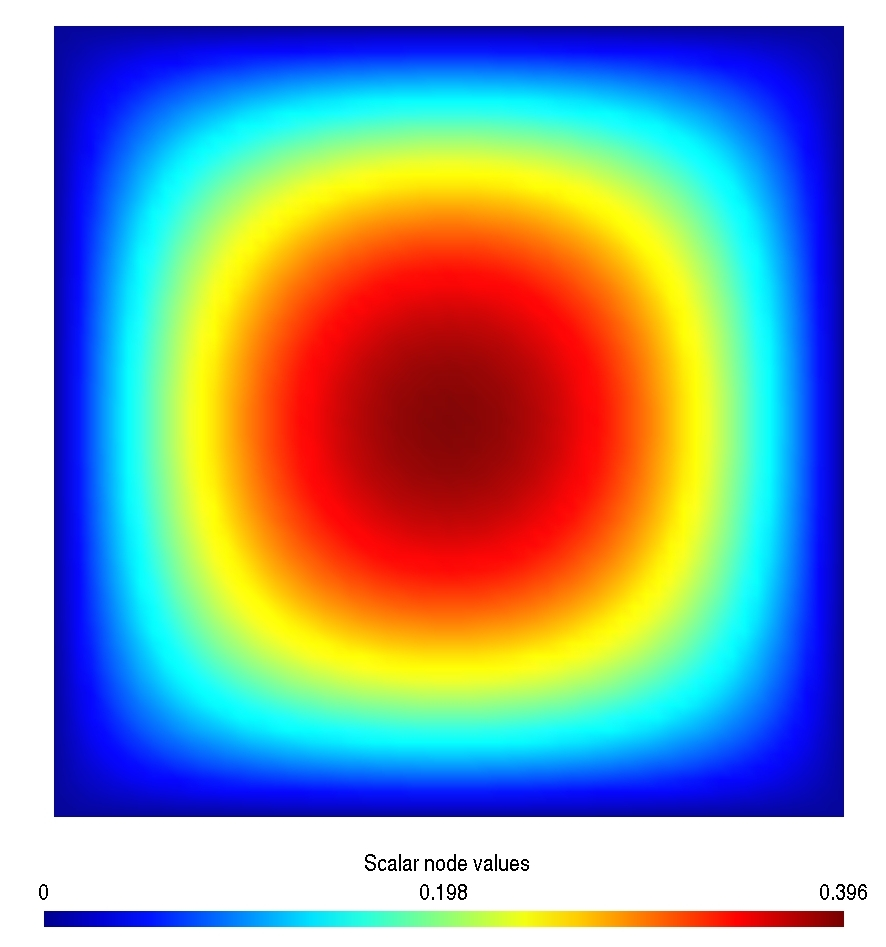
\includegraphics[scale=0.2]{images/bratu.jpg}}
\subfigure{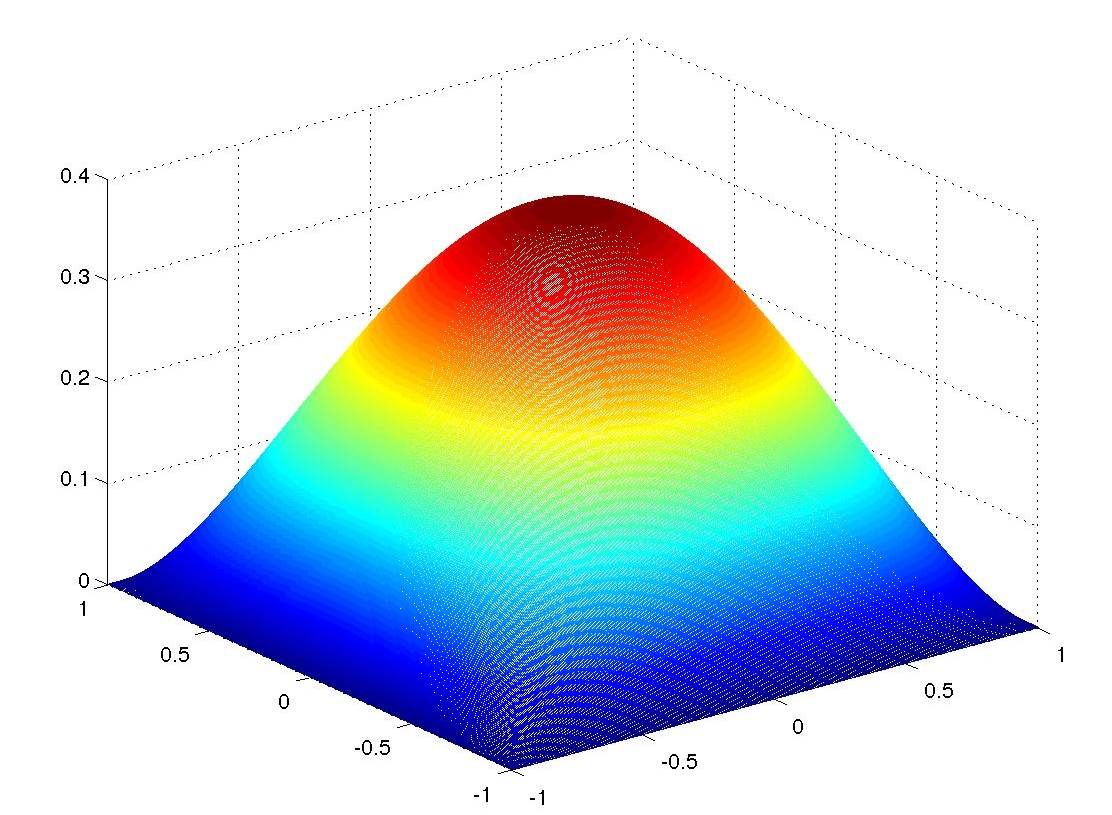
\includegraphics[scale=0.2]{images/bratu_surf.jpg}}
\caption{Discrete solution of the Bratu equation.}\label{fig:bratu}
\end{figure}

In Fig.(\ref{fig:bratu_norm}) we plot the dependence of the residual from the initial guess. More precisely, the x-axis shows the iteration step of the nonlinear solver while the y-axis shows, in logarithmic scale, the value of the residual $\|F(u^{(n)})\|_{L^2(\Omega)}$. We report three different initial guess: $u^{(0)}(\mathbf{x})=0$ in red, $u^{(0)}(\mathbf{x})=1$ in green and $u^{(0)}(\mathbf{x})=0$ in blue. The initial guess is set only on the degrees of freedom of the problem while on the Dirichlet boundary are set the right values of the solution.

\begin{figure}
\centering
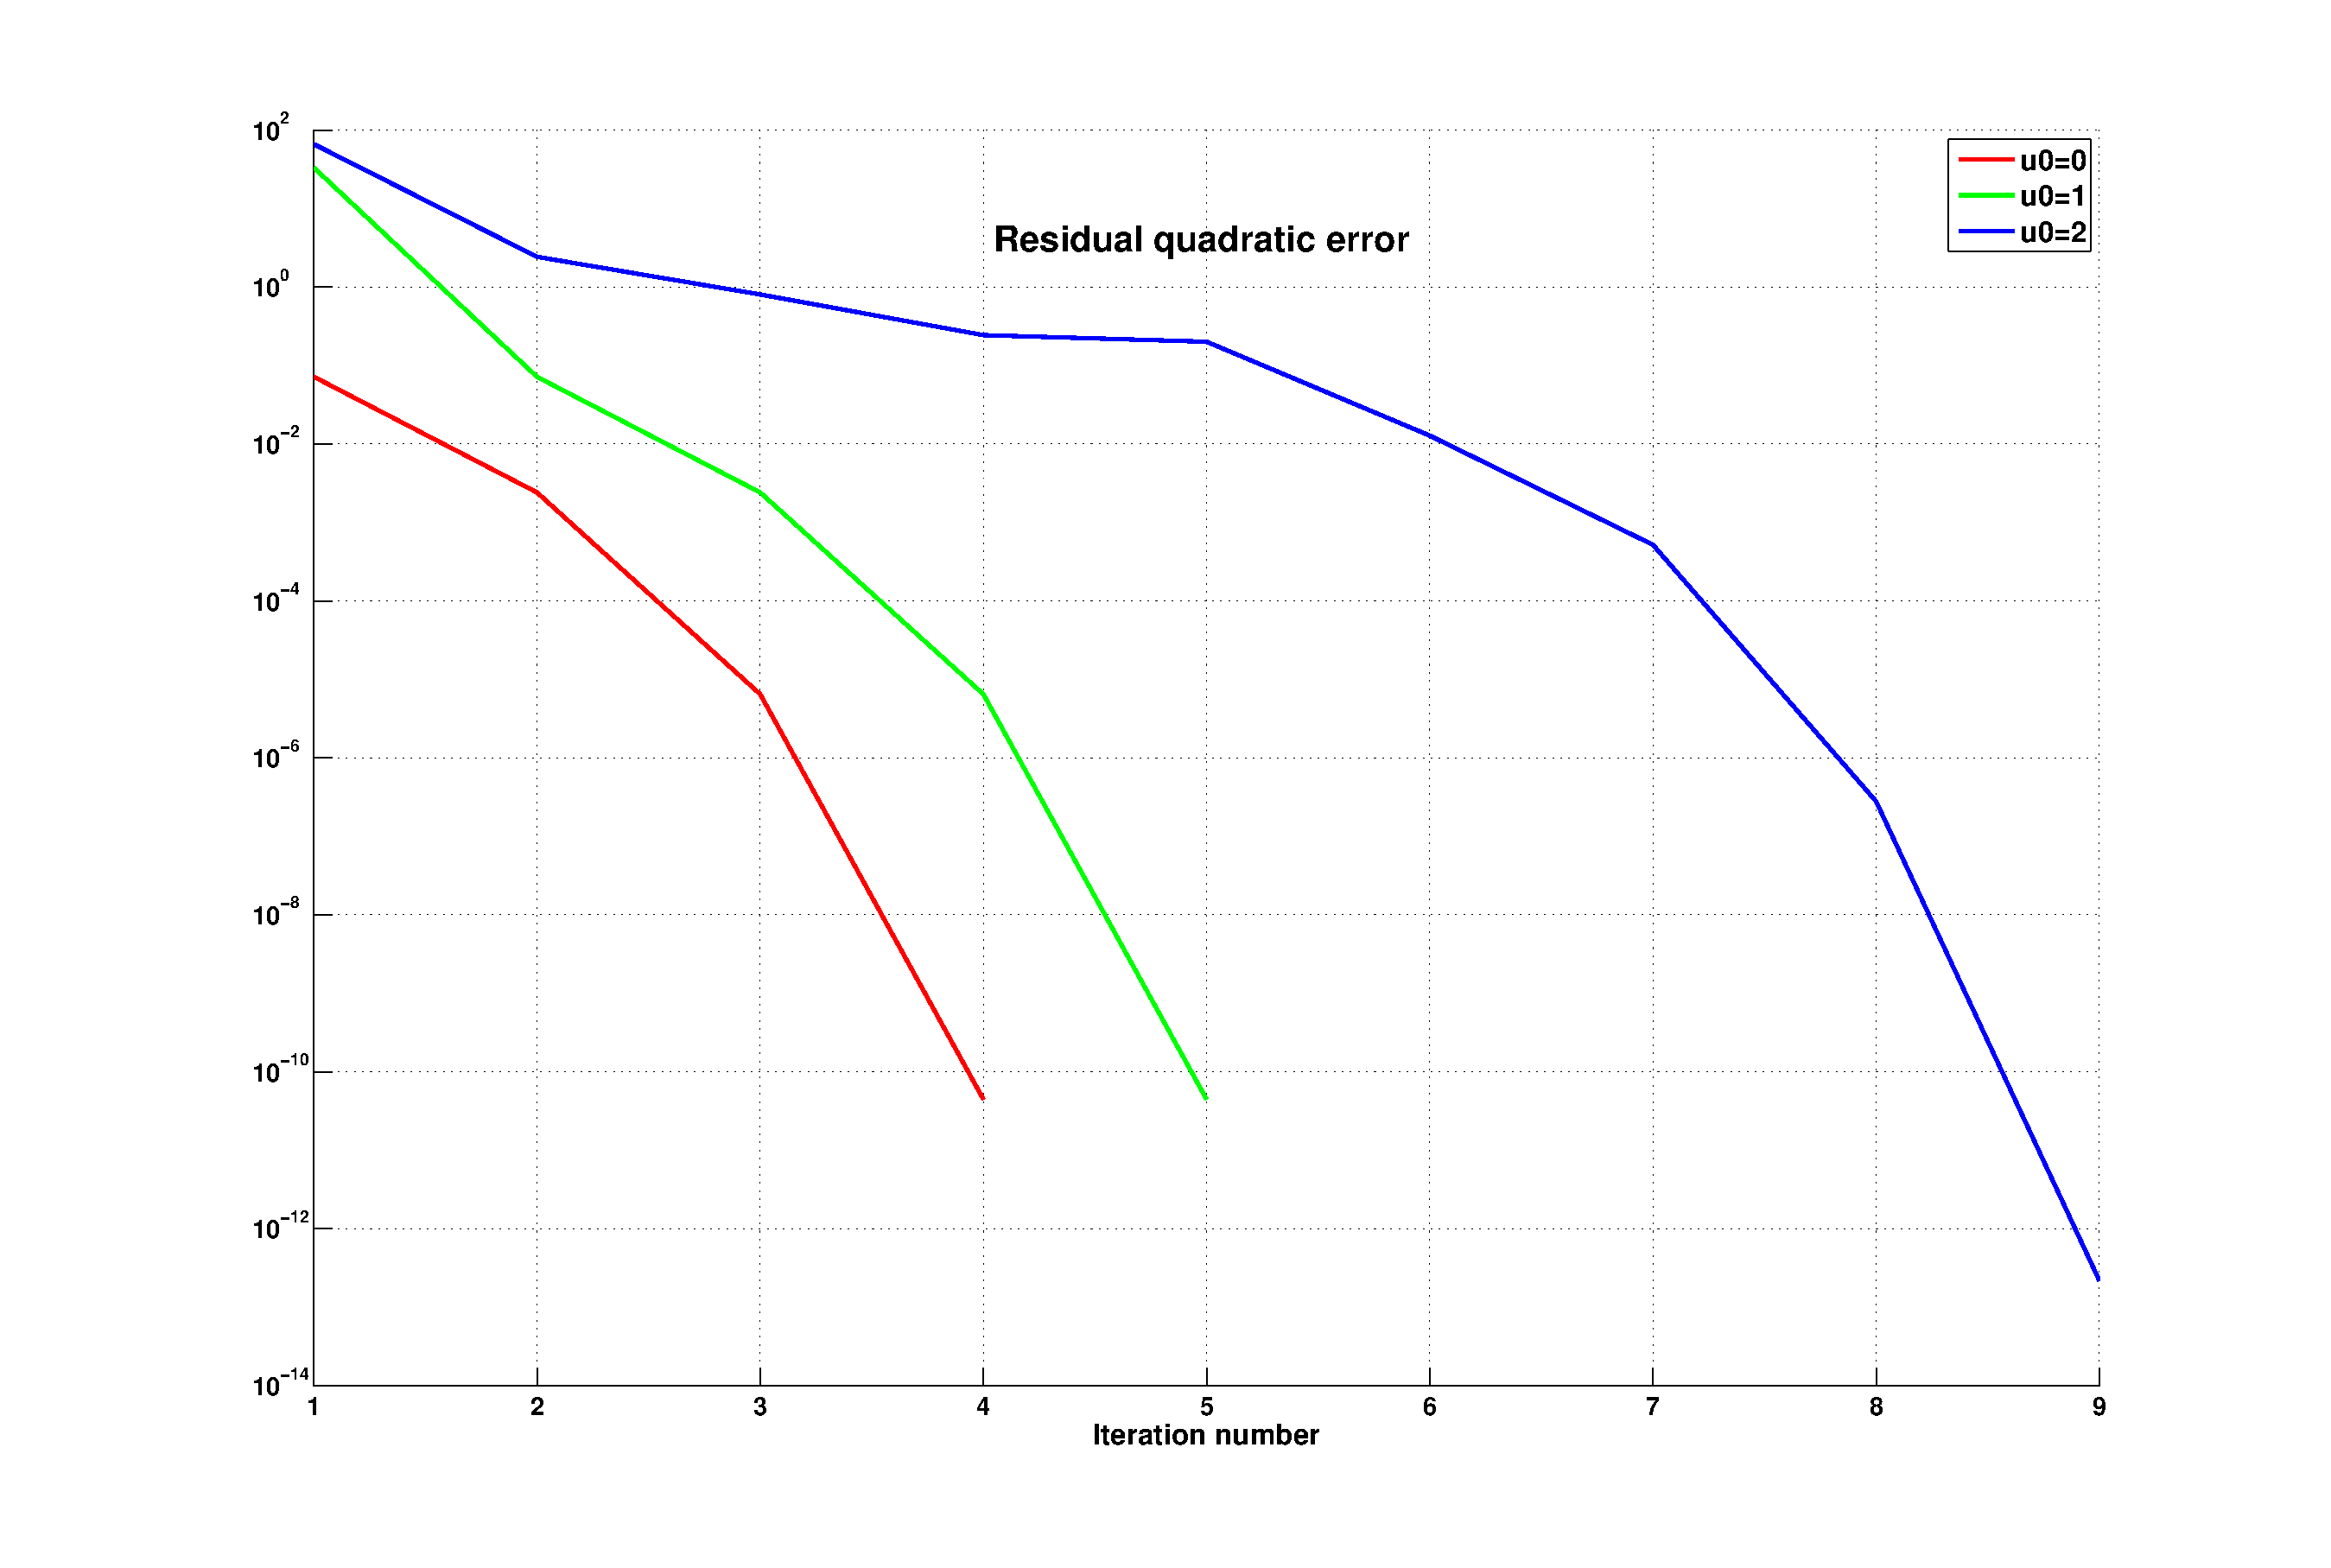
\includegraphics[scale=0.3]{images/bratu_norm.eps}
\caption{Dependence of the residual $\|F(u^{(n)})\|_{L^2(\Omega)}$ from the initial guess.}\label{fig:bratu_norm}
\end{figure}

We can notice that, in both 3 cases, the desired tolerance is reached way before the maximum number of iterations but also that varying a little the initial guess, the number of iteration can change considerably. The nonlinear solver part, which is built over the linear solver code, reaching the tolerance of the residual in a small number of iteration, works fine in the test case.

\subsection{Nonlinear Grad-Shavranov}
We now solve our problem, cmp. Eq.(\ref{eq:compact_equlibrium}), in the mirror domain shown in Fig.(\ref{fig:mirror_domain}) with the following parallel pressure profile
\begin{equation}
  f(r,z,B,\psi)=p_0\big(1-\frac{\psi^2}{\psi^2_0}\big).
\end{equation}
Using this profile, the problem (\ref{eq:compact_equlibrium}) becomes
\begin{equation}
  \begin{cases}
    -\Delta^*\psi-p_0\:r^2\:\big(1-\frac{\psi^2}{\psi^2_0}\big)=0 & \mathrm{in}\:\Omega\\
    \psi(z,\gamma(z))=2\\
    \psi(0,r)=\psi(1,r)\\
    \nabla\psi(0,r)=\nabla\psi(1,r)
  \end{cases}
\end{equation}
which is nonlinear. Using the formalism introduce in Sec.(\ref{subsec:newton_method}) we have the following non linear functional $F$ defined as
\begin{equation}
  F(\psi)=\int_\Omega \bigg(r\:\nabla \psi \cdot\nabla v+2\:v\:\partial_r\psi-r^3\:p_0\big(1-\frac{\psi^2}{\psi^2_0}\big)\bigg)\mathrm{d}\Omega
\end{equation}
and its Gateaux derivative is
\begin{equation}
  \mathcal{F}(\psi)\delta \psi=\int_\Omega \bigg(r\:\nabla \delta\psi \cdot\nabla v+2\:v\:\partial_r\delta\psi+2\frac{p_0}{\psi^2_0}\:r^3v\:\psi\delta\psi\bigg)\mathrm{d}\Omega.
\end{equation}

The discrete formulation of the problem is
\begin{equation}
  \begin{split}
    &F\big(\psi^{(k)}(\mathbf{x})\big)=\\
    &\sum_m \bigg\{\sum_n w_n\:\mathbf{F}_m^r(\mathbf{\hat{x}}_n)\hat{\nabla}\hat{\psi}^{(k)}(\mathbf{\hat{x}}_n)J_{\mathbf{F}_m}^{-1}(\mathbf{\hat{x}}_n)J_{\mathbf{F}_m}^{-T}(\mathbf{\hat{x}}_n)\hat{\nabla}\hat{\phi}_i(\mathbf{\hat{x}}_n)|\det(J_{\mathbf{F}_m}(\mathbf{\hat{x}}_n))| +\\
    &+2\:\sum_n w_n[\frac{\partial\hat{x}}{\partial r},\frac{\partial\hat{y}}{\partial r}]_{\big|_{\mathbf{\hat{x}}_n}}\hat{\nabla} \hat{\psi}^{(k)}(\mathbf{\hat{x}}_n)\:\hat{\phi}_i(\mathbf{\hat{x}}_n)|\det(J_{\mathbf{F}_m}(\mathbf{\hat{x}}_n))|+\\
    &-\sum_n w_n\:p_0\:\mathbf{F}_m^r(\mathbf{\hat{x}}_n)^3 \bigg(1-\bigg(\frac{\hat{\psi}^{(k)}}{\psi_0}\bigg)^2\bigg)\hat{\phi}_i(\mathbf{\hat{x}}_n)|\det(J_{\mathbf{F}_m}(\mathbf{\hat{x}}_n))|\bigg\}=0, \qquad\forall i\in\mathcal{I};
  \end{split}
\end{equation}
\begin{equation}
  \begin{split}
    &\mathcal{F}(\psi^{(k)})\bigg(\sum_j\delta \psi_j\phi_j(\mathbf{x})\bigg)=\\
    &\sum_m \bigg\{\sum_j \delta\psi_j \sum_n w_n\:\mathbf{F}_m^r(\mathbf{\hat{x}}_n)\hat{\nabla}\hat{\phi}_j(\mathbf{\hat{x}}_n)J_{\mathbf{F}_m}^{-1}(\mathbf{\hat{x}}_n)J_{\mathbf{F}_m}^{-T}(\mathbf{\hat{x}}_n)\hat{\nabla}\hat{\phi}_i(\mathbf{\hat{x}}_n)|\det(J_{\mathbf{F}_m}(\mathbf{\hat{x}}_n))| +\\
    &+2\:\sum_j\delta\psi_j\sum_n w_n[\frac{\partial\hat{x}}{\partial r},\frac{\partial\hat{y}}{\partial r}]_{\big|_{\mathbf{\hat{x}}_n}}\hat{\nabla} \hat{\phi}_j(\mathbf{\hat{x}}_n)\:\hat{\phi}_i(\mathbf{\hat{x}}_n)|\det(J_{\mathbf{F}_m}(\mathbf{\hat{x}}_n))|+\\
    &+2\sum_j\delta\psi_j\sum_n w_n\:\frac{p_0}{\psi_0^2}\mathbf{F}_m^r(\mathbf{\hat{x}}_n)^3\hat{\phi}_i(\mathbf{\hat{x}}_n)\hat{\psi}^{(k)}(\mathbf{\hat{x}}_n)\hat{\phi}_j(\mathbf{\hat{x}}_n)|\det(J_{\mathbf{F}_m}(\mathbf{\hat{x}}_n))|\bigg\}=0, \qquad\forall i\in\mathcal{I},
  \end{split}
\end{equation}
and is defined in the class \verb|gradshavranov.h|.
\medskip

The mesh used and the settings of the linear solver are the same of the ones used in Sec.(\ref{subsec:ex_gs_operator}). We set the tolerance of the nonlinear solver equal to $10^{-7}$ and the maximum number of iteration is 50. We choose $\psi^2_0=1$. The plots of the numerical solution are reported in Fig.(\ref{fig:gs}) where the first plot has $p_0=1$ while the second $p_0=1000$.

\begin{figure}
\centering
\subfigure{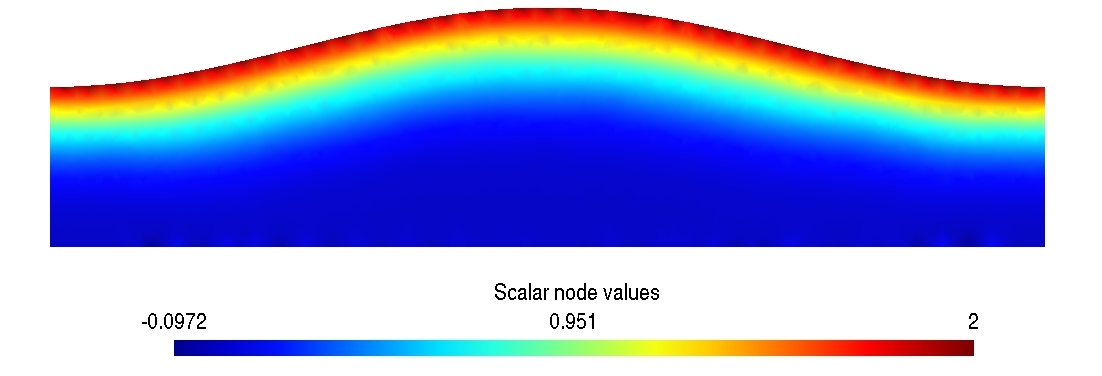
\includegraphics[scale=0.32]{images/gs.jpg}}
\subfigure{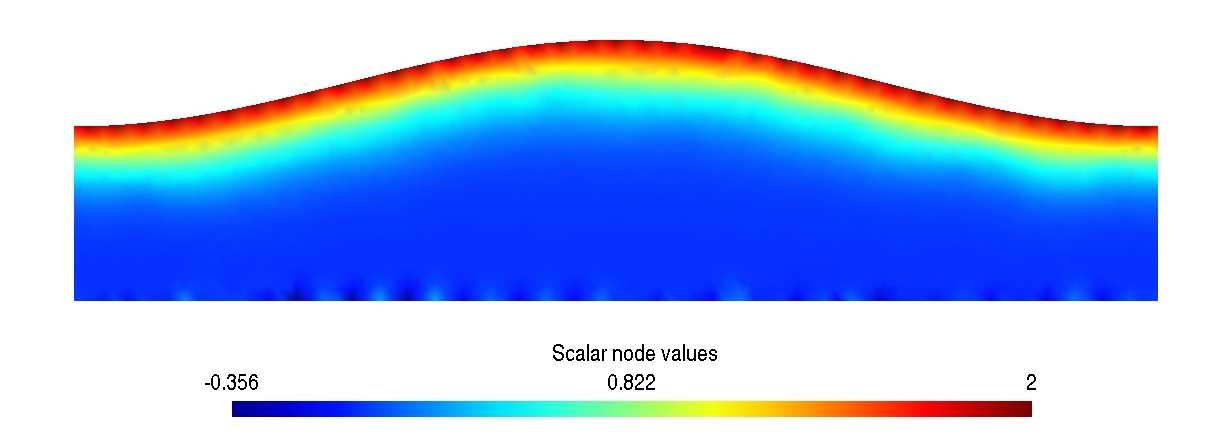
\includegraphics[scale=0.29]{images/gs_1000.jpg}}
\caption{Discrete solution of the nonlinear Grad-Shavranov problem with $p_0=1$ and $p_0=1000$.}\label{fig:gs}
\end{figure}

We can notice that when $p_0=1$ the solution is very close to the one shows in Sec.(\ref{subsec:ex_gs_operator}). That is not surprising indeed the function $ f(r,z,B,\psi)$ is multiplied by $r^3\propto10^{-3}$ therefore the nonlinearity influences the solution by a factor proportional to $\frac{1}{1000}$; instead, in the second case, the linear and the nonlinear term have the same order of magnitude and the solution is strongly influenced by the nonlinear term.
